\documentclass[10pt, aspectratio=169]{beamer}

\mode<presentation>{


%%%% ТЕМЫ %%%%
% \usetheme{Berlin} %++main++
% \usetheme{Boadilla} %+
% \usetheme{CambridgeUS} %-
\usetheme{Madrid} %+
% \usetheme{Montpellier} % свобода в названиях, секциях и подсекциях
% \usetheme{Pittsburgh} %минимализм
% \usetheme{Szeged} %классический, без авторов, с нижней строкой


%%%% ЦВЕТА %%%%
% \usecolortheme{beaver} %+осень
% \usecolortheme{crane} %+осень?
% \usecolortheme{dolphin}
% \usecolortheme{dove} %+беленький
% \usecolortheme{seagull} %+business
\usecolortheme{seahorse} %+winter
% \usecolortheme{whale} %+winter
% \usecolortheme{spruce} %+spring


%%%% ДРУГИЕ НАСТРОЙКИ %%%%
%\setbeamertemplate{footline} % To remove the footer line in all slides uncomment this line
%\setbeamertemplate{footline}[frame number] % To replace the footer line in all slides with a simple slide count uncomment this line
\setbeamertemplate{navigation symbols}{} % Чтобы удалить символы навигации со дна всех скользких скользких
\setbeamercovered{transparent} % Раскрывает серые анимации (полезные для дизайна, но могут быть прокомментированы при передаче окончательного документа)
% Использовать шрифт вспышки везде
\usefonttheme{serif}
}


\usepackage[T2A]{fontenc}                   %!? закрепляет внутреннюю кодировку LaTeX
\usepackage[utf8]{inputenc}                 %!  закрепляет кодировку utf8
\usepackage[english,russian]{babel}         %!  подключает русский и английский
\usepackage[margin=1.8cm, left=30mm, right=15mm, top=20mm, bottom=20mm]{geometry}         %!  фиксирует оступ на 2cm

\usepackage[unicode, pdftex]{hyperref}      %!  оглавление для панели навигации по PDF-документу + гиперссылки

\usepackage{cite}                           %   цитирование несколько источников
\bibliographystyle{unsrt}

\usepackage{amsthm}                         %!  newtheorem и их сквозная нумерация
\usepackage{hypcap}                         %?  адресация на картинку, а не на подпись к ней
\usepackage{caption}                        %-  позволяет корректировать caption 
\usepackage{fancyhdr}                       %   добавить верхний и нижний колонтитул
\usepackage{wrapfig}                        %!  обтекание таблиц и рисунков

\usepackage{amsmath}                        %!  |
\usepackage{amssymb,textcomp, esvect,esint} %!  |важно для формул 
\usepackage{amsfonts}                       %!  математические шрифты
\usepackage{mathrsfs}                       %  добавит красивые E, H, L
% \usepackage{ulem}                           %!  перечеркивание текста
\usepackage{abraces}                        %?  фигурные скобки сверху или снизу текста
\usepackage{pifont}                         %!  нужен для крестика
\usepackage{cancel}                         %!  аутентичное перечеркивание текста
\usepackage{esvect}                         %  добавит вектора стрелочками

\usepackage{graphicx}                       %?  графическое изменение текста
\usepackage{indentfirst}                    %   добавить indent перед первым параграфом
\usepackage{xcolor}                         %   добавляет цвета
\usepackage{enumitem}                       %!  задание макета перечня.

% \usepackage{booktabs}                       %!  добавляет книжные линии в таблицы
% \usepackage{multirow}                       %   объединение ячеек в таблицах
\usepackage{tikz}                           %!  высокоуровневые рисунки (кружочек)
% \usepackage{import}                         %   |
% \usepackage{xifthen}                        %   |
% \usepackage{pdfpages}                       %   | вставка рисунков pdf_tex
% \usepackage{transparent}                    %   |

\usepackage{bbm}                            %   добавляет \mathbbm{1}
\usepackage{subfigure}
% базовая подстройка
\renewcommand{\d}{\, d}
\renewcommand{\leq}{\leqslant}
\renewcommand{\geq}{\geqslant}



% специфично под документ
\newcommand{\dC}{\,{}^\circ\textnormal{С}}
\newcommand{\un}[1]{\,\text{#1}}
\newcommand{\meas}[3]{(#1 \pm #2)\,\text{#3}}

% авторские команды
\newcommand{\vc}[1]{\boldsymbol{#1}}
\newcommand{\1}{\mathbbm{1}}
\newcommand{\T}{^{\textnormal{T}}}
\newcommand{\con}{^{\dag}}
\newcommand{\sub}[2]{#1_{\textnormal{#2}}}
\newcommand{\vp}{\vphantom{\dfrac{1}{2}}}

% операторы (просто прямой текст)
\renewcommand{\Im}{\mathop{\mathrm{Im}}\nolimits}
\renewcommand{\Re}{\mathop{\mathrm{Re}}\nolimits}
% \renewcommand{\P}{\mathop{\mathrm{P}}\nolimits}
% \newcommand{\E}{\mathop{\mathrm{E}}\nolimits}
% \newcommand{\D}{\mathop{\mathrm{D}}\nolimits}
% \newcommand{\cov}{\mathop{\mathrm{cov}}\nolimits}
\newcommand{\diag}{\mathop{\mathrm{diag}}\nolimits}
\newcommand{\card}{\mathop{\mathrm{card}}\nolimits}
\newcommand{\grad}{\mathop{\mathrm{grad}}\nolimits}
\renewcommand{\div}{\mathop{\mathrm{div}}\nolimits}
\newcommand{\rot}{\mathop{\mathrm{rot}}\nolimits}
\newcommand{\Ker}{\mathop{\mathrm{ker}}\nolimits}
\newcommand{\spec}{\mathop{\mathrm{spec}}\nolimits}
\newcommand{\sign}{\mathop{\mathrm{sign}}\nolimits}
\newcommand{\tr}{\mathop{\mathrm{tr}}\nolimits}
\newcommand{\rg}{\mathop{\mathrm{rg}}\nolimits}
\newcommand{\const}{\textnormal{const}}


% цветной текст
\newcommand{\red}[1]{\textcolor{red}{#1}}
\newcommand{\green}[1]{\textcolor{urlcolor}{#1}}
\newcommand{\blue}[1]{\textcolor{ublue}{#1}}


% символы
\newcommand{\cmark}{\text{\ding{51}}}
\newcommand{\xmark}{\text{\ding{55}}}


% подгрузка pdf_tex картинок
% \newcommand{\incfig}[1]{%
%     \def\svgwidth{\columnwidth}
%     \import{./figures/}{#1.pdf_tex}
% }


% специфично к квантам
\newcommand{\ket}[1]{\left| #1 \right\rangle}
\newcommand{\bra}[1]{\left\langle #1 \right|}

% \newcommand{\dppp}{\frac{d^3 p}{(2 \pi \hbar)^3}}

\DeclareDocumentCommand{\bk}{m o m}{
    \IfNoValueTF{#2}{\langle #1 | #3 \rangle}{\langle #1 | #2 | #3 \rangle}
}

\title[Оптимизация в МОЛ]{Оптимизация количества атомов тулия \\ в
магнито-оптической ловушке}


\author[Хоружий Кирилл]{Хоружий Кирилл \texorpdfstring{
\\
\phantom{}\\
группа <<Квантовые симуляторы и интегрированная фотоника>>\\
\phantom{}\\
Научный руководитель: Акимов А. В. \\
Научный консультант: Цыганок В. В.
}{} 
}
\institute[РКЦ, МФТИ]


\let\tg\undefined %костыль связанный с русским языком и tg

\setbeamertemplate{caption}[numbered]

\begin{document}
\maketitle


\frame{
	% ВВЕДЕНИЕ
% -- введение (демонстрирует понимание студентом научного контекста и умение
% представлять свое исследование широкой аудитории, содержит постановку
% задачи с обзором научной литературы и с указанием предмета, целей, объектов,
% инструментов и значения исследования, а также актуальности работы и личного
% вклада автор, краткий обзор разделов ВКР);










 \frametitle{Ультрахолодные газы}
}
\frame{
	\begin{figure}[h]
    \centering
    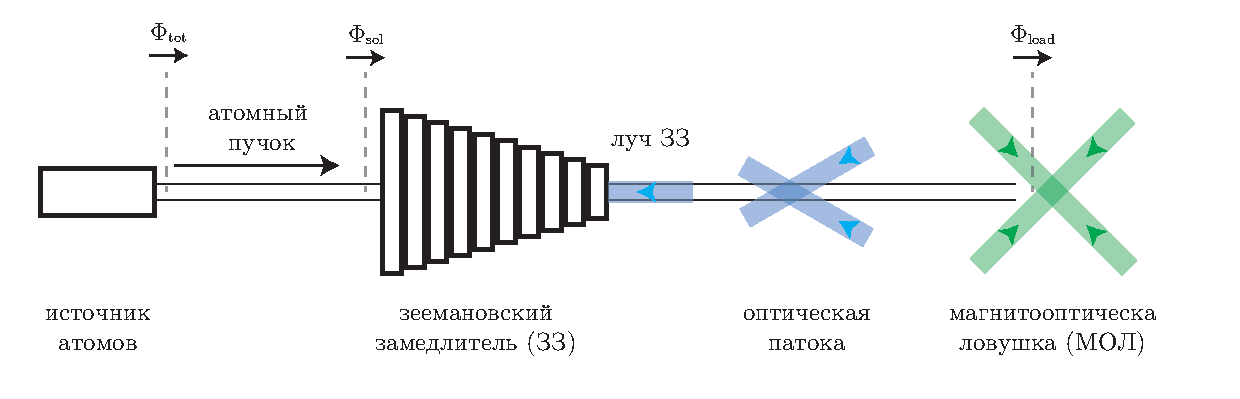
\includegraphics[width=1.0\textwidth]{../MOT/figs/sheme.pdf}
    \caption{Принципиальная схема установки}
\end{figure}


\begin{figure}[h]
    \centering
    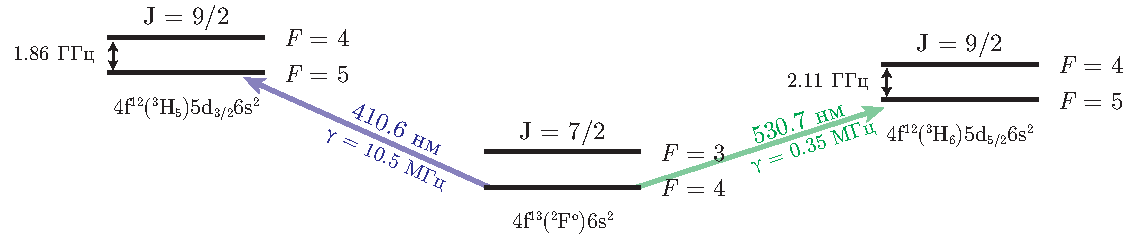
\includegraphics[width=1.0\textwidth]{../MOT/figs/tm_pres.pdf}
    \caption{Используемые в эксперименте атомные переходы}
\end{figure}


 \frametitle{Общая схема охлаждения}
}
\frame{
	


\begin{minipage}{0.65\textwidth}

\begin{figure}[ht]
    \centering
    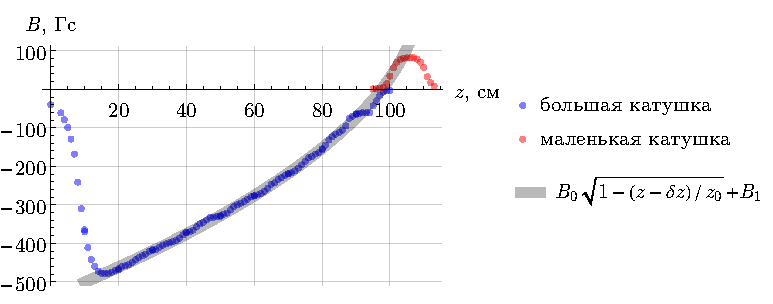
\includegraphics[width=0.9\textwidth]{../MOT/figs/Bz_v2.pdf}
    \caption{Зависимость магнитного поля внутри зеемановского замедлителя от координаты $z$. Ток маленькой катушки $\sub{I}{small} = 17\,$А, ток большой катушки $\sub{I}{big} = 35\,$А.}
\end{figure}


\end{minipage}
\hfill
\begin{minipage}{0.31\textwidth}

Тормозящая сила:
\begin{equation*}
    F = \frac{\hbar k \Gamma}{2} \frac{s}{1+s+4({\delta}+k v)^2/\Gamma^2}
\end{equation*}

\phantom{42}

Эффект Доплера:\\
\phantom{42} \hfill
$1\,\text{м}/\text{с} \sim 2\,\text{МГц}$

При этом: \\
\phantom{42} \hfill
$\Gamma \sim 10\,\text{МГц}$

Замедление \\
\phantom{4} 
от $150\,\text{м}/\text{с}$ до $\sub{v}{slow} \sim 30\,\text{м}/\text{с}$

\phantom{42}



Необходима подстройка резонанса магнитным полем:
\begin{equation*}
    \delta \to \delta + \mu B / \hbar
\end{equation*}


\end{minipage} \frametitle{Зеемановский замедлитель I}
}
\frame{
	

% \begin{tikzpicture}[remember picture,overlay]    \draw[seahorse] (10.5,0.75) -- (10.5,-6.75); \end{tikzpicture}


\begin{minipage}{0.65\textwidth}

\begin{figure}[ht]
    \centering
    \subfigure[]{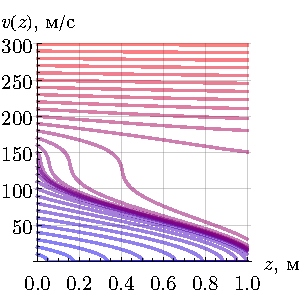
\includegraphics[scale=0.7]{../MOT/figs/vz_v2.pdf}}
    \hspace{5 mm} 
    \subfigure[]{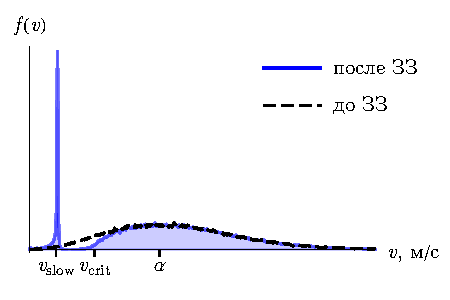
\includegraphics[scale=0.7]{../MOT/figs/vdist_v5.pdf}}
    % zeeman_sim_v2
    \caption{a) Зависимость скорости атомов от координаты в зеемановском замедлителе  для различных начальных скоростей. б) Характерное преобразование распределения атомов по скоростям после замедления. }
\end{figure}


\end{minipage}
\hfill
\begin{minipage}{0.31\textwidth}

Тормозящая сила:
\begin{equation*}
    F = \frac{\hbar k \Gamma}{2} \frac{s}{1+s+4({\delta}+k v)^2/\Gamma^2}
\end{equation*}

\phantom{42}

Уравнение движения:
\begin{equation*}
    \frac{d v}{d t} = \frac{F}{m},
    \hspace{0.1cm} \overset{v \d t = \d z}{\Leftrightarrow}  \hspace{0.1cm}
    \frac{d v}{d z} = \frac{F(v, z)}{m \, v(z)}
\end{equation*}



\end{minipage} \frametitle{Зеемановский замедлитель II}
}
\frame{
	



\begin{minipage}{0.65\textwidth}
\begin{figure}[ht]
    \centering
    \rotatebox{90}{\hspace{8mm}\scalebox{0.8}{$B_0=700\un{Гс}$ \hspace{16 mm} $B_0=300\un{Гс}$}}
    \hspace{1 mm} 
    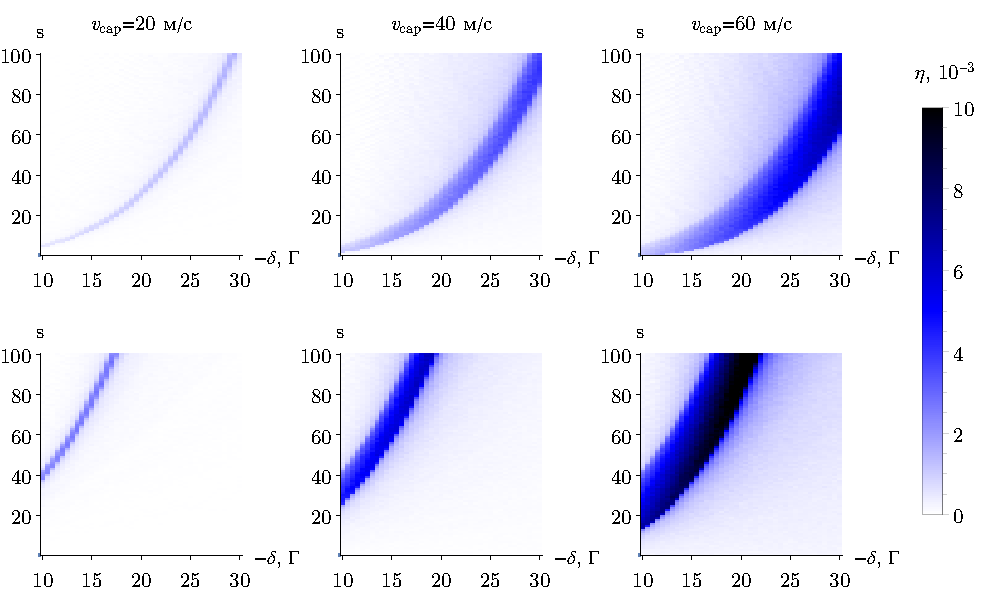
\includegraphics[width=0.94\textwidth]{../MOT/figs/etas_v4.pdf}
    \caption{Зависимость эффективности работы замедлителя $\eta$ от отстройки луча ЗЗ $\delta$, параметра насыщения $s$ для двух различных значений амплитуды магнитного поля в ЗЗ}
\end{figure}

\end{minipage}
\hfill
\begin{minipage}{0.31\textwidth}



Загрузка в МОЛ: $\ v < \sub{v}{cap}$

\phantom{42}

$\eta = \frac{\sub{\Phi}{load}}{\sub{\Phi}{sol}}$ -- эффективность ЗЗ

\phantom{42}

\begin{figure}[h]
    \centering
    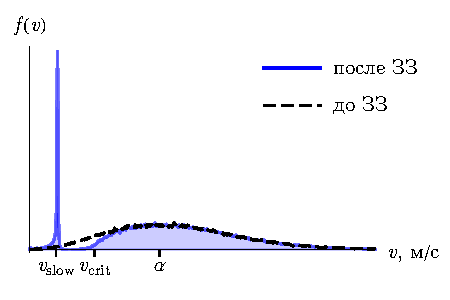
\includegraphics[scale=0.66]{../MOT/figs/vdist_v5.pdf}
    \caption{Преобразование распределения атомов по скоростям после ЗЗ}
    %\label{fig:}
\end{figure}


\end{minipage} \frametitle{Зеемановский замедлитель III}
}
\frame{
	\begin{minipage}{0.68\textwidth}




\only<1>{

Сила в МОЛ:
	\begin{equation*}
		\vc{F} = \frac{\hbar \vc{k} \Gamma}{2}\left(
			\frac{s}{1+s+4\left(\frac{2\pi \delta - \vc{k} \vc{v}}{\Gamma}\right)^2}-
			\frac{s}{1+s+4\left(\frac{2\pi \delta + \vc{k} \vc{v}}{\Gamma}\right)^2}
		\right)
	\end{equation*}

	\begin{figure}[h]
    \centering
    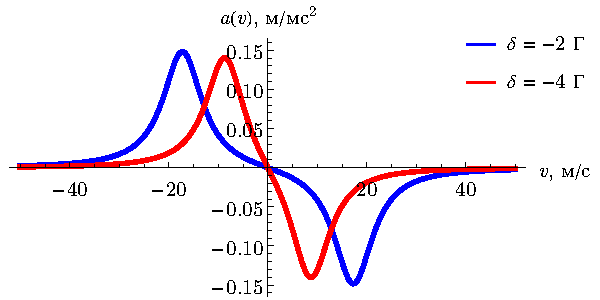
\includegraphics[width=0.8\textwidth]{../MOT/figs/motF.pdf}
    \caption{Зависимость ускорения от силы светового давления, действующей на движущийся атом от его скорости}
    %\label{fig:}
\end{figure}
}

\only<2>{

Сила в МОЛ:
	\begin{equation*}
		\vc{F} = \frac{\hbar \vc{k} \Gamma}{2}\left(
			\frac{s}{1+s+4\left(\frac{2\pi \delta - \vc{k} \vc{v}}{\Gamma}\right)^2}-
			\frac{s}{1+s+4\left(\frac{2\pi \delta + \vc{k} \vc{v}}{\Gamma}\right)^2}
		\right)
	\end{equation*}

	Магнитное поле $\Rightarrow$ эффект Зеемана:
	\begin{equation*}
		\vc{B} = \beta (-x,\,  -y,\, 2z)\T/2,
		\hspace{10 mm} 
		\Delta E = - \vc{B} \vc{\mu},
		\hspace{5 mm} 
		\delta \to \delta + \Delta E /\hbar
	\end{equation*}

	\phantom{42}



	Движение в МОЛ $\sim$ затухающий осциллятор:
	\begin{equation*}
		\vc{F}(\vc{r}, \vc{v}) = -\alpha \vc{v} - \varkappa \vc{r}
	\end{equation*}

	с коэффициентами
	\begin{equation*}
			\varkappa = \frac{-\delta}{\Gamma/2\pi}\frac{8 \subt{\mu}{B} \beta k s}{\left(1+s+4\left(\frac{2\pi \delta}{\Gamma}\right)^2\right)^2},
			\hspace{5 mm} 
			\alpha = \frac{-\delta}{\Gamma} \frac{8 \hbar k^2 s}{\left(1+s+4\left(\frac{2\pi \delta}{\Gamma}\right)^2\right)^2},
	\end{equation*}

}



\end{minipage}
\hfill
\begin{minipage}{0.31\textwidth}

\begin{figure}[h]
    \centering
    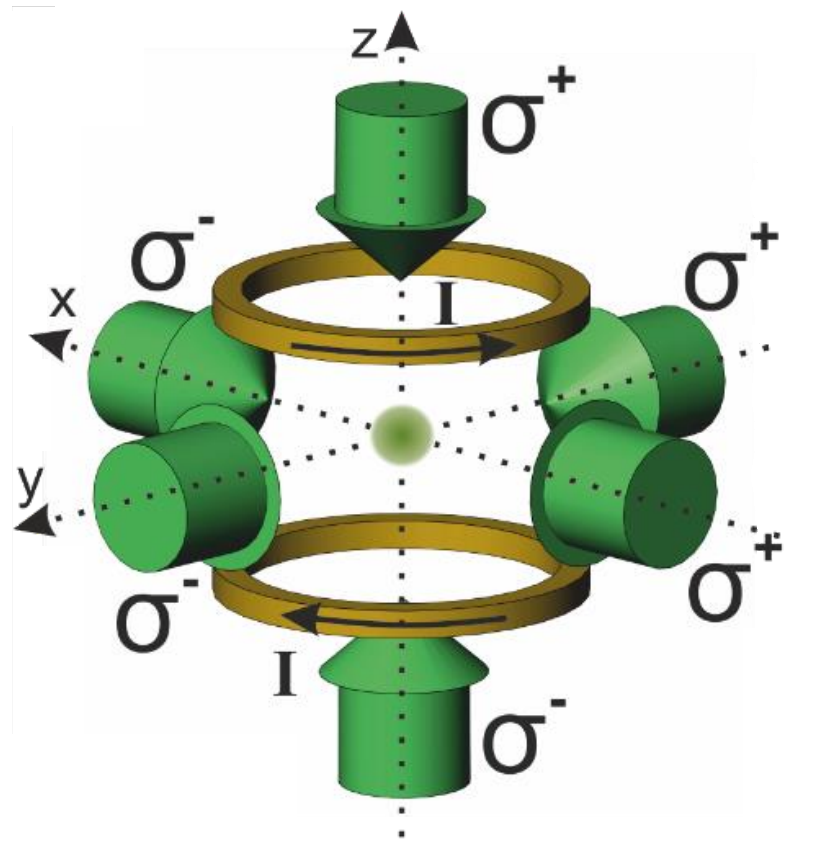
\includegraphics[width=1.0\textwidth]{../MOT/figs/mot.png}
    \caption{Схема лучей МОЛ}
    %\label{fig:}
\end{figure}

\end{minipage}



 \frametitle{Магнито-оптическая ловушка (МОЛ)}
}
\frame{
	% \begin{figure}[ht]
%     \centering
%     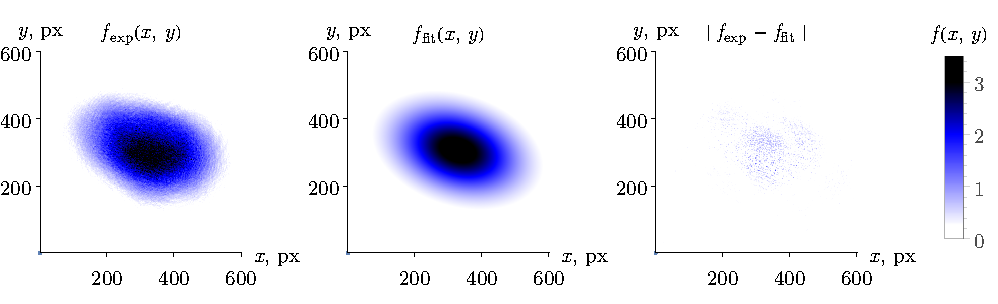
\includegraphics[width=0.6\textwidth]{../MOT/figs/fit_mot_v2.pdf}
%     \caption{Экспериментально сфотографированное распределение 
%     атомов $\sub{f}{exp}$ и аппроксимация распределения атомов $\sub{f}{fit}$
%     }
% \end{figure}

\begin{minipage}{0.68\textwidth}
Закон Бугера-Ламберта-Бера:
\begin{equation*}
    \frac{d I}{d z} = - \sigma n I,
    \hspace{10 mm} 
    \sigma = \frac{\sigma_0}{1+I/I_s + 4 (\delta/\Gamma)^2},
\end{equation*}


Распределение интенсивности:
\begin{equation*}
    \sub{f}{exp} = \ln\left(\frac{\subt{I}{D}}{I_0}\right) + \frac{\subt{I}{D} - I_0}{I_s} = \sigma_0 \int n(x, y, z) \d z.
\end{equation*}

\begin{figure}[ht]
    \centering
    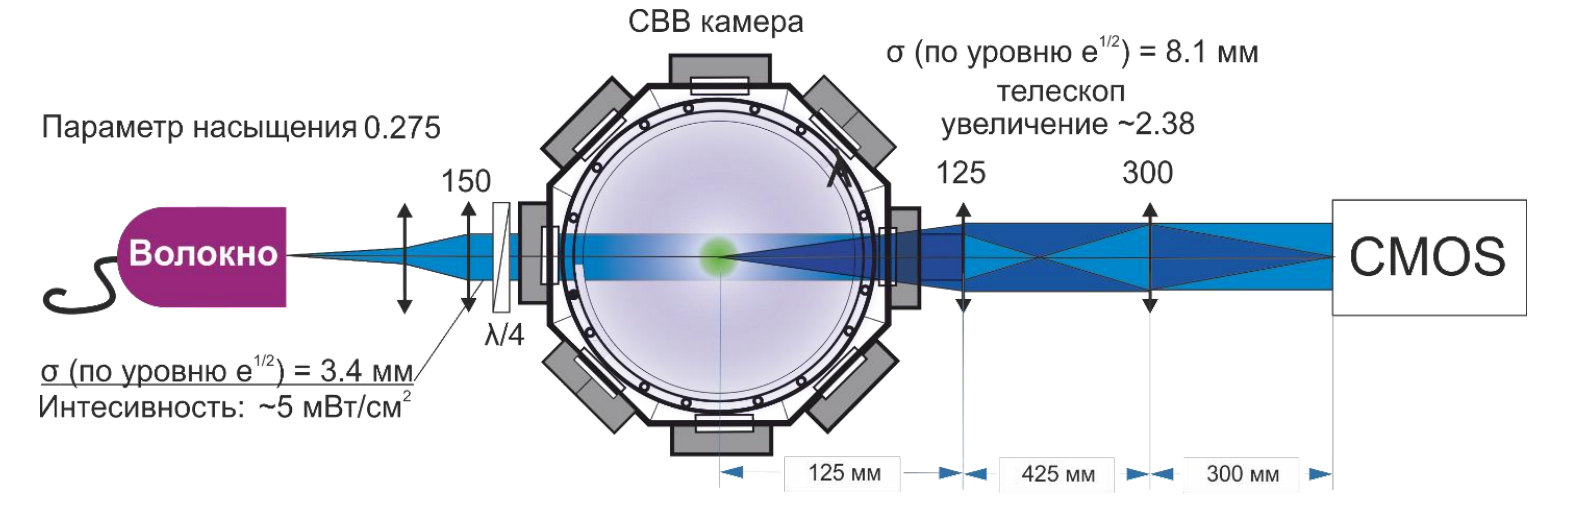
\includegraphics[width=0.9\textwidth]{../MOT/figs/detect.png}
    \caption{Схема детектирования атомов}
\end{figure}
\end{minipage}
\hfill
\begin{minipage}{0.31\textwidth}

$\subt{I}{D}$ -- фотография без атомов

$\sub{I}{0}$ -- фотография с атомами

$\sub{I}{s}$ -- интенсивность насыщения

\begin{figure}[h]
    \centering
    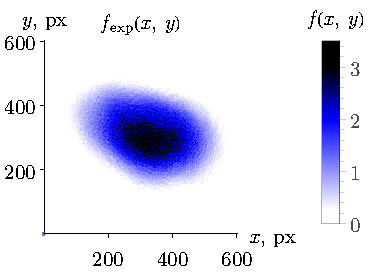
\includegraphics[width=0.99\textwidth]{../MOT/figs/fit_mot_v4.pdf}
    \caption{Фото распределения}
    %\label{fig:}
\end{figure}


\end{minipage} \frametitle{Фотографирование атомов}
}
\frame{
	\begin{minipage}{0.6\textwidth}

Аппроксимация распределения:
\begin{equation*}
    \sub{f}{fit}(x, y) = B+A \exp\left(
        - \left(\frac{\tilde{x}}{\sigma_1}\right)^2 - \left(\frac{\tilde{y}}{\sigma_2}\right)^2
    \right)
\end{equation*}


\end{minipage}
\hfill
\begin{minipage}{0.31\textwidth}

Полное число атомов:
\begin{equation*}
\boxed{
	N = \pi A \sigma_1 \sigma_2
}
\end{equation*}

\end{minipage}


\begin{figure}[h]
    \centering
    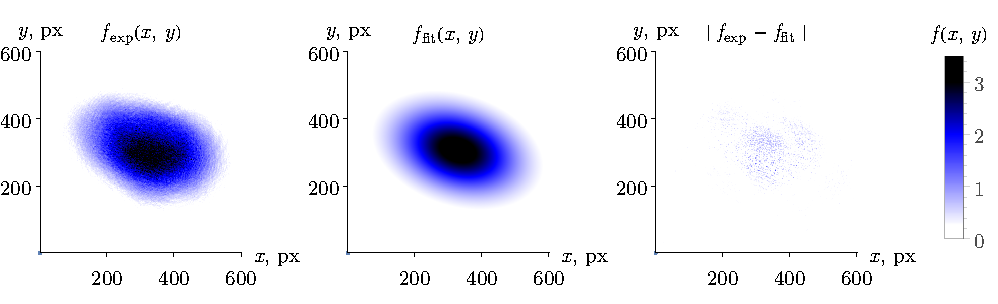
\includegraphics[width=0.8\textwidth]{../MOT/figs/fit_mot_v2.pdf}
    \caption{Экспериментально сфотографированное распределение атомов $\sub{f}{exp}$, аппроксимация распределения атомов гауссовой функцией $\sub{f}{fit}$ и остатки аппроксимации $|\sub{f}{exp} - \sub{f}{fit}|$}
    %\label{fig:}
\end{figure}
 \frametitle{Количество атомов в МОЛ}
}
\frame{
	Динамика количества атомов в МОЛ:
\begin{equation*}
	\frac{d N}{d t} = \sub{\Phi}{load} - \cancel{\gamma N} - \beta N^2
	\hspace{0.5cm} \Rightarrow \hspace{0.5cm}
	N(t) = \sqrt{\frac{\sub{\Phi}{load}}{\beta}} \left(1-e^{-t \sqrt{\beta \sub{\Phi}{load}}}\right)
\end{equation*}




\begin{minipage}{0.6\textwidth}


\begin{figure}[h]
    \centering
    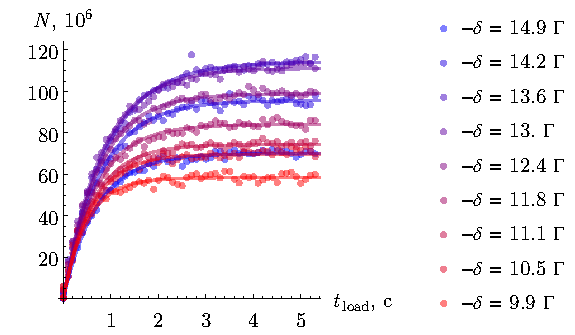
\includegraphics[width=0.8\textwidth]{../MOT/figs/motload_v2.pdf}
    \caption{Динамика загрузки МОЛ для различных значений отстройки $\delta$ лучей МОЛ}
    %\label{fig:}
\end{figure}

\end{minipage}
\hfill
\begin{minipage}{0.35\textwidth}

\begin{figure}[h]
    \centering
    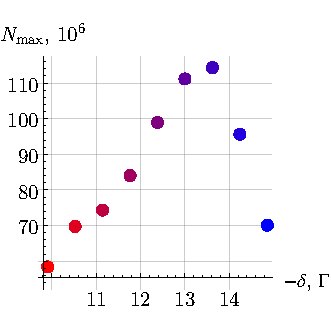
\includegraphics[width=0.8\textwidth]{../MOT/figs/motload2_v2.pdf}
    \caption{Зависимость максимального числа атомов в МОЛ от величины отстройки $\delta$ лучей МОЛ}
\end{figure}

\end{minipage} \frametitle{Загрузка МОЛ: оптимизация отстройки лучей МОЛ}
}
\frame{
	\begin{figure}[ht]
    \centering
    \subfigure[]{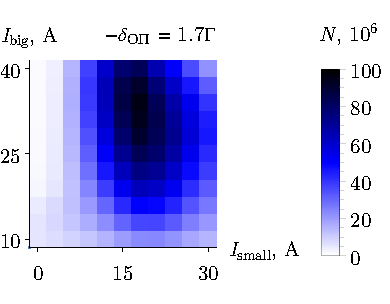
\includegraphics[width=0.3\textwidth]{../MOT/figs/IZ1.pdf}}
    \hspace{10 mm} 
    \subfigure[]{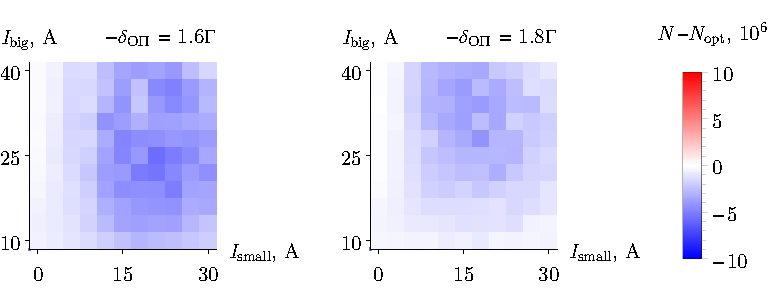
\includegraphics[width=0.6\textwidth]{../MOT/figs/IZ2.pdf}}
    \caption{a) Зависимость количества загруженных за 5с в МОЛ атомов от величины токов малой и большой катушки ЗЗ. Зависимость снята  при оптимальной отстройке лучей ОП $\subt{\delta}{ОП}$. 
    б) Зависимость количества загруженных за 5с при оптимальной отстройке лучей ОП в МОЛ атомов от величины токов малой и большой катушки ЗЗ. Зависимость снята при $\subt{\delta}{ОП}$ большей и меньшей оптимального значения в $\subt{\delta}{ОП} = 9.4 \Gamma$.}
\end{figure}

 \frametitle{Загрузка МОЛ: оптимизация токов зеемановского замедлителя}
}
\frame{
	\begin{minipage}{0.65\textwidth}
    \vspace{-1mm}

    \begin{figure}[h]
        \centering
        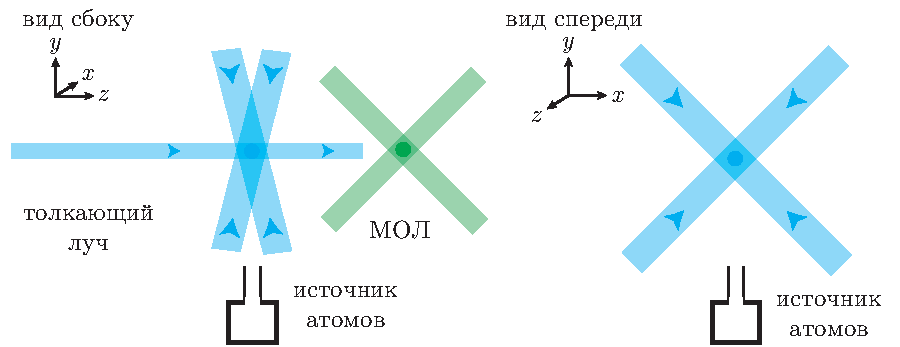
\includegraphics[width=0.9\textwidth]{../MOT/figs/2dmot_v3.pdf}
        \vspace{1mm}
        \caption{Принципиальная схема лучей 2D-МОЛ}
        \label{fig:2dmots}
    \end{figure}

    \vspace{-8mm}

    \begin{figure}[h]
        \centering
        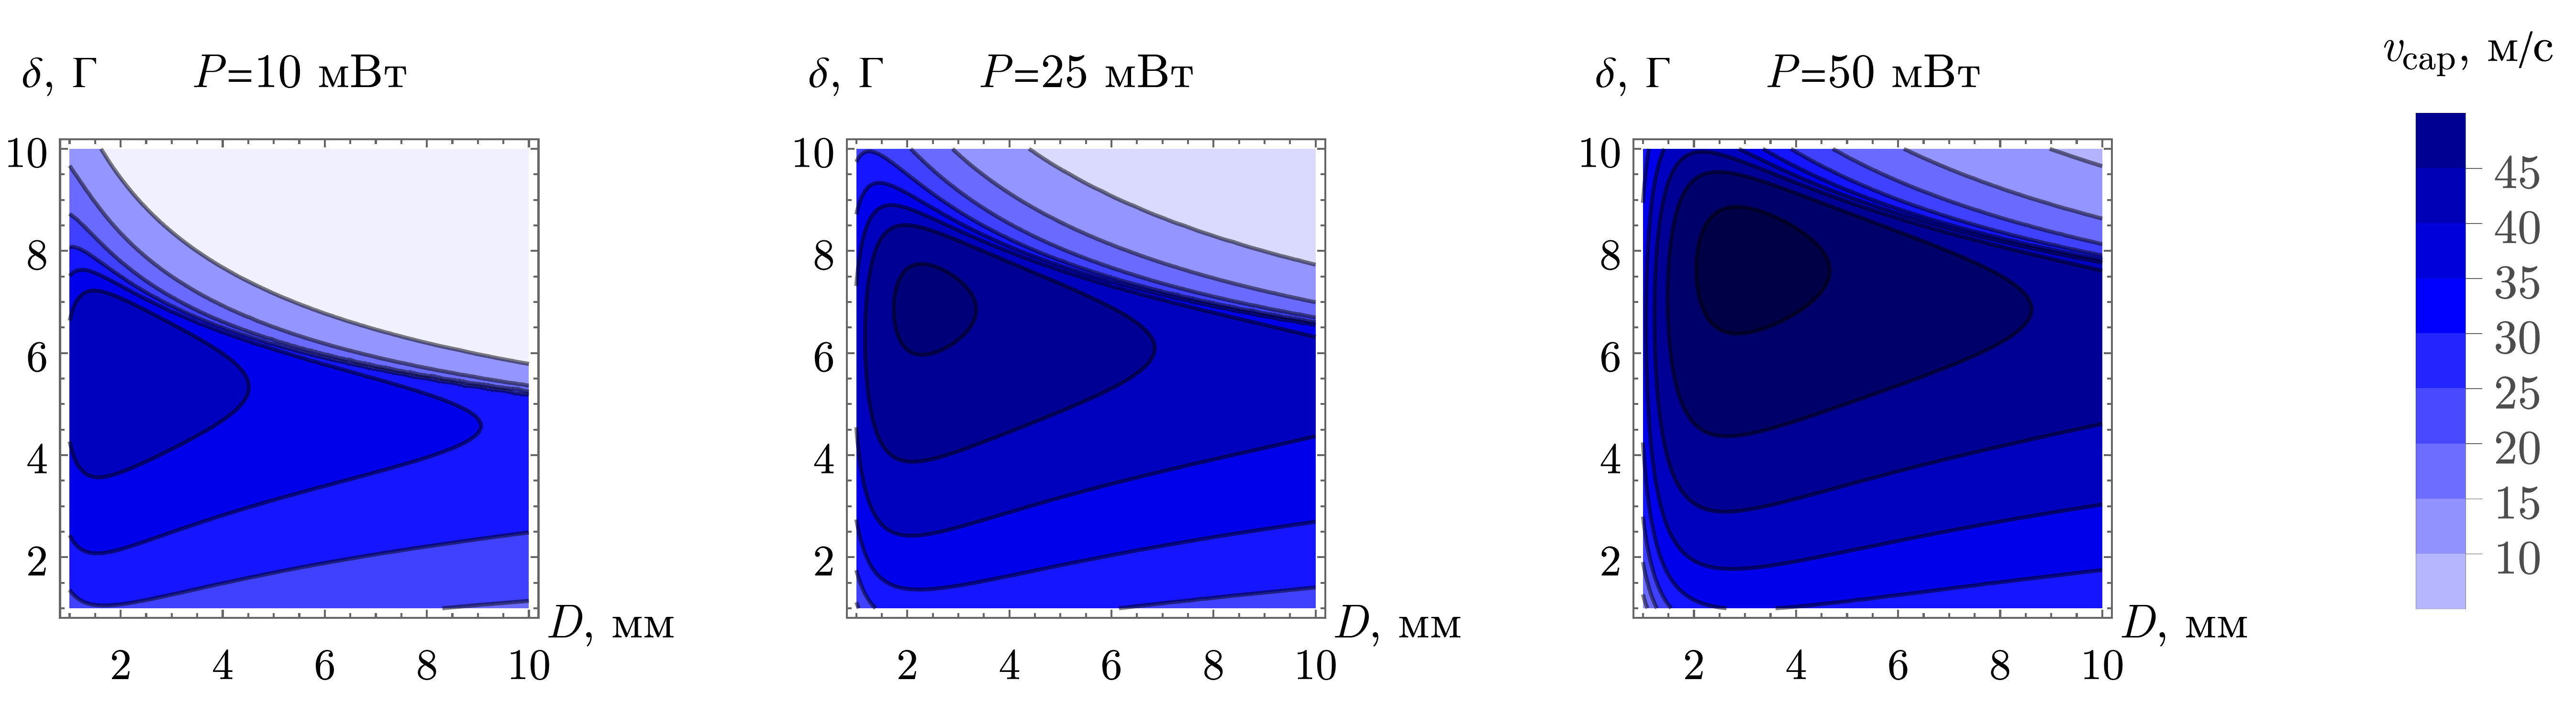
\includegraphics[width=1.0\textwidth]{../MOT/figs/vcap2d_delta-Ds.png}
        \caption{Зависимость скорости захвата 2D-МОЛ для различных мощностей от отстройки $\delta$ лучей 2D-МОЛ и размера $D$ пучков}
    \end{figure}
\end{minipage}
\hfill
\begin{minipage}{0.31\textwidth}

Загрузка МОЛ: \vspace{-3mm}
\begin{align*}
    % \sub{\Phi}{load} &\propto \sub{\Phi}{tot} \int_{0}^{\vcap} v^3 e^{-v^2/\alpha^2} \d v \\
    \sub{\Phi}{load} &\propto  \sub{\Phi}{sol} \left(\frac{\sub{v}{\textcolor{blue}{cap}}}{\alpha}\right)^4
\end{align*}


Скорости захвата: \vspace{-3mm}
\begin{equation*}
    m \int_{\vcap}^{0} \frac{v}{F(v)} \d v = D
\end{equation*}


Критическое расстояние: \vspace{-3mm}
\begin{equation*}
    \sub{l}{крит} \sim \sqrt{\frac{\sub{h}{крит} \sub{v}{\textcolor{green}{cap}}^2}{g}} \sim 1\,\text{м}
\end{equation*}


\phantom{42}

При $T \sim 700 \dC$: \\ 
$\sub{\Phi}{load}(\sub{v}{\textcolor{blue}{cap}} = 40\,\text{м/c}) \sim 10^8\,\text{c}^{-1}$

\end{minipage} \frametitle{2D-MOЛ}
}
\frame{
	% Тут что-то в духе

%  было: ...


%  стало: ...


%  Стало лучше!

%  

\begin{itemize}
	\iitem{Построена модель ЗЗ. Моделированием методом Монте-Карло определена зависимость системы от параметров.}
	\iitem{Оптимизацией работы ЗЗ, ОП и МОЛ удалось уменьшить температуру с $730\dC$ до $680\dC$, сохранив загрузку МОЛ $\sub{\Phi}{load}$ на исходном уровне. Это увеличило время непрерывной работы установки в 5 раз: с 2 месяцев до 10 месяцев.} 
	\iitem{Подготовлена альтернатива ЗЗ: 2D-МОЛ. Произведены основные оценки необходимые для работы 2D-МОЛ. После 2D-МОЛ мы можем получить загрузку МОЛ $\sub{\Phi}{load}$ на исходном уровне, таким образом 2D-МОЛ является компактной перспективной заменой ЗЗ.}
\end{itemize}



 \frametitle{Заключение}
}
\frame{
	\centering
\LARGE{Спасибо за внимание!} \frametitle{}
}


\end{document}



